\section{Results}
\label{sec:results}

Unless stated otherwise, results refer to the \nDaysConfFour{} four-parameter days of the \nSitesConf{} confirmation sites, with the development value (\nDaysDevFour{} days at \nSitesDevFour{} sites) for comparison, and intervals are site-clustered 95\% bootstrap intervals.

\subsection{Cost of a record within tolerance (RQ1)}
\label{sec:need}
A four-parameter day needed a median of \needMedConf{} bytes of values (\needMedConfCI{}), that is, nine values or two messages; the development median was the same (\needMedDev{} bytes). The 90th percentile was \needPninetyConf{} bytes, the 99th percentile \needPnnConf{} bytes, and the largest day needed \needMaxConf{} bytes (Fig.~\ref{fig:need}). The record held \valueShareConf{} of the readings and \byteShareConf{} of the bytes of the raw readings (median), and \oneMsgConf{} of days fitted a single message. With each site weighted equally, the median was \needSiteEqConf{} bytes; the \nDaysConfFewer{} record days with one to three parameters needed a median of \needMedConfFewer{} bytes. On the development data, the share of readings kept rose from \shareFiveDev{} at 5-minute sampling to \shareFifteenDev{} at 15 minutes and \shareSixtyDev{} at hourly sampling, because a smooth signal sampled often needs few values, whereas an hourly record leaves little to omit. The need was largest in summer: the share of days fully certified with six messages per day fell from \monthMaxConf{} in winter to \monthMinConf{} in July and August (Supplementary Fig. S1).

\begin{figure}[t]
\centering
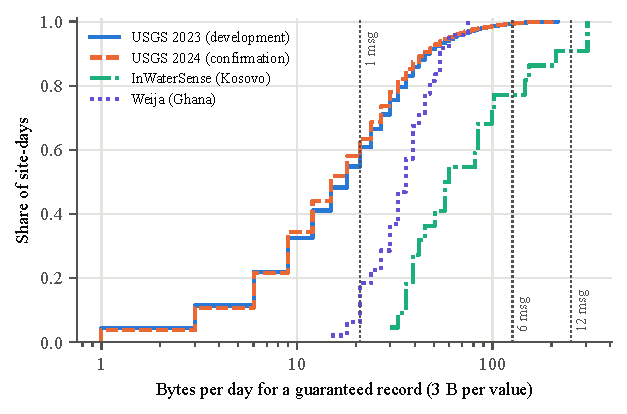
\includegraphics[width=0.6\textwidth]{figs/need_ecdf.pdf}
\caption{Bytes of values needed for a record within tolerance, per four-parameter day. Vertical lines mark the capacity of one, two, and six messages.}
\label{fig:need}
\end{figure}

\subsection{Delivery without knowledge of the channel (RQ2)}
\label{sec:delivery}
Table~\ref{tab:delivery} and Fig.~\ref{fig:delivery} compare the designs at six messages per day. At an independent loss probability of 0.3, the record-first code fully certified \gCodeIidConf{} of days (\gCodeIidConfCI{}); site means ranged from \gSiteMinConf{} to \gSiteMaxConf{}, with a median of \gSiteMedConf{} (Supplementary Table S2). It exceeded record-first repetition by \dRepIidConf{} (\dRepIidConfCI{}), the channel-blind fixed-$K$ code by \dFixedIidConf{} (\dFixedIidConfCI{}), the reliable-link design by \dRelIidConf{}, tag practice by \dTagIidConf{}, and every $k$-th reading by \dEveryIidConf{}. The advantage over repetition shrank as loss became burstier: \dRepBurConf{} (\dRepBurConfCI{}) with bursts of three messages and \dRepBsixConf{} (\dRepBsixConfCI{}) with bursts of six, where both designs lose whole runs of messages whatever they carry. The code was never below repetition on any day, as Proposition 2 requires.

\begin{table}[t]
\centering
\caption{Days fully certified, $G_{\mathrm{cert}}$, at six and twelve messages per day (confirmation sites; 95\% intervals).}
\label{tab:delivery}
\small
\begin{tabularx}{\textwidth}{@{}>{\raggedright\arraybackslash}X*{4}{>{\raggedright\arraybackslash}p{2.3cm}}@{}}
\toprule
Design & Independent, $p = 0.1$ & Independent, $p = 0.3$ & Bursty, $p = 0.3$ & Bursts of 6, $p = 0.3$ \\
\midrule
\tableinput{tables/delivery.tex}
\bottomrule
\end{tabularx}
\end{table}

\begin{figure}[t]
\centering
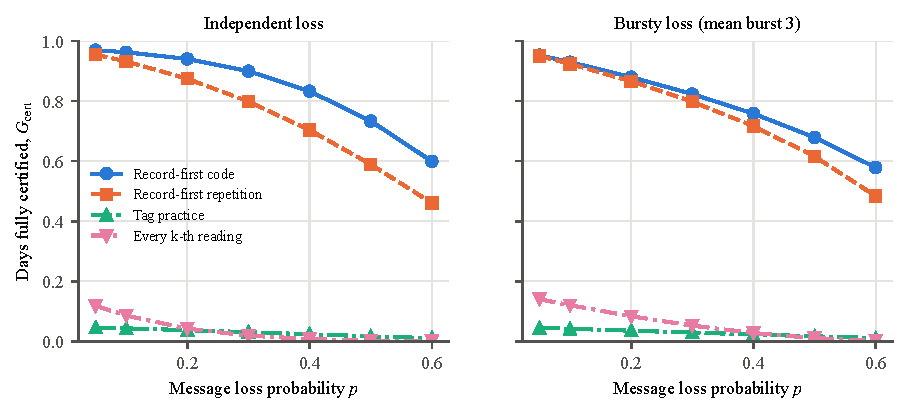
\includegraphics[width=\textwidth]{figs/delivery.pdf}
\caption{Days fully certified against the message loss probability, six messages per day (confirmation sites).}
\label{fig:delivery}
\end{figure}

Three analyses on the development data explain the ranking:
\begin{itemize}
  \item Channel knowledge: a code of fixed dimension needs the loss rate to choose $K$. Chosen without it, it lost up to \regretFixedDev{} against the same code tuned for the true channel; tuned for a loss probability of 0.1 and used at 0.6, it lost \mismatchMaxDev{} (Fig.~\ref{fig:mismatch}). The record-first code was at least as good as the tuned fixed code on all 15 channels and four tiers. A server that estimated the channel from the message indices of a 28-day pilot and reconfigured the node lost at most \pilotLossDev{}: feasible, but unnecessary with record-first coding.
  \item Content versus transmission policy: sending the record's units with the tags' random policy cost \tagPolicyDev{} against interleaved repetition, whereas sending broken-stick points instead of the record cost a further \tagContentDev{}: tag practice lost mainly because its points are not chosen against a tolerance.
  \item Other codes and orders: a systematic random linear (fountain-style) code matched Reed--Solomon to within 0.001; interleaving repetition copies made no difference under independent loss but added \interleaveDev{} under bursty loss.
\end{itemize}

\begin{figure}[t]
\centering
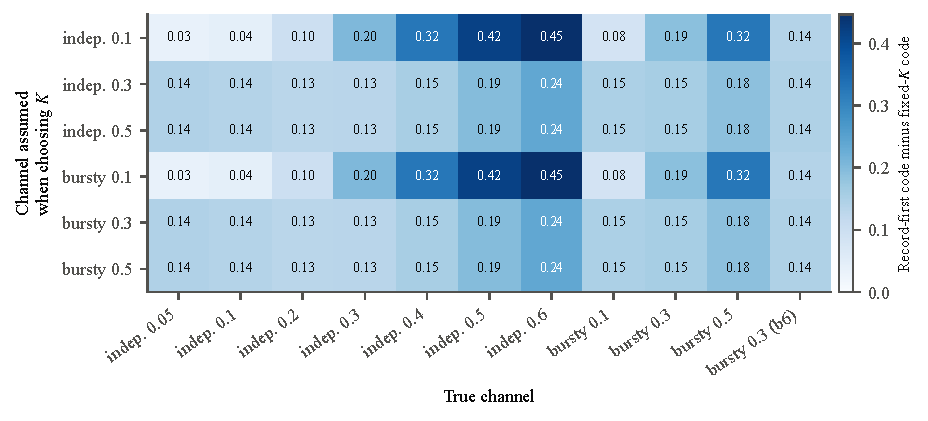
\includegraphics[width=\textwidth]{figs/mismatch.pdf}
\caption{Advantage of the record-first code over a fixed-$K$ code chosen for an assumed channel (rows) and used on the true channel (columns); six messages per day, development data.}
\label{fig:mismatch}
\end{figure}

\subsection{Message plans, buffering, and plan sizing (RQ3)}
\label{sec:plans}
A site met the target when at least 90\% of its days were fully certified within seven days. With six messages per day, \sitesSixIidConf{} confirmation sites met it under independent loss of 0.3 and \sitesSixBurConf{} under bursty loss; with twelve messages, \sitesTwelveIidConf{} and \sitesTwelveBurConf{}; with 24, all. With twelve messages per day, the code certified \gTwelveIidConf{} of days under independent loss and \gTwelveBurConf{} under bursty loss.

Buffering did not help (development data). A node that carried a first-in, first-out backlog of records into later blocks was never better by more than 0.007 than sending each day's record on the next day at six or more messages per day, and at one message per day its backlog grew without bound and \droppedDev{} record days exceeded the frame's 63-day limit. Rotating the units of the last seven days, as satellite tags do, gave time diversity: under bursts of six messages it certified \rotBsixDev{} of days within a week against \dailyBsixDev{} for the next-day code, but only \rotGoneDev{} by the next day (Fig.~\ref{fig:multiday}).

\begin{figure}[t]
\centering
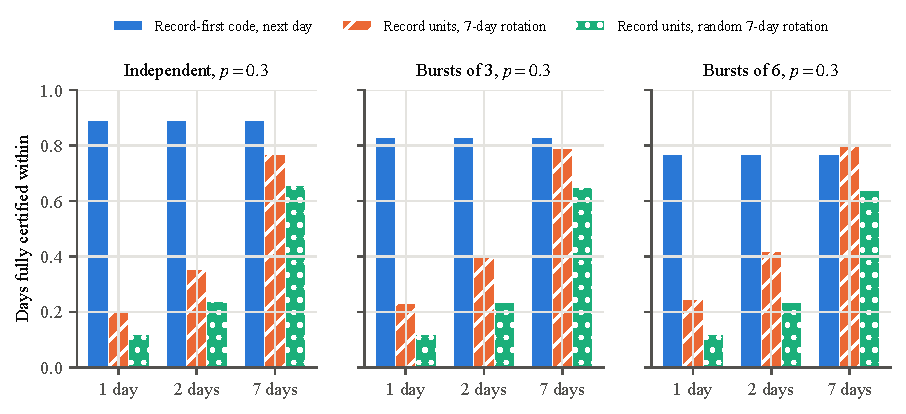
\includegraphics[width=\textwidth]{figs/multiday.pdf}
\caption{Days fully certified within one, two, and seven days for the next-day record-first code and two seven-day rotations of the record's units; six messages per day, development test sites.}
\label{fig:multiday}
\end{figure}

A plan chosen as the smallest tier whose 28-day pilot certified at least 90\% of days within a week was sufficient for the rest of the year in \sizeSuffConf{} (\sizeSuffConfCI{}) of \sizePilotsConf{} site-pilots started in any month, and it over-provisioned by more than one tier in \sizeOverConf{}. Pilots in the quiet season underestimated the summer need: December pilots were sufficient in \sizeDecConf{} of cases.

\subsection{Environmental decisions (RQ4)}
\label{sec:env}
Fig.~\ref{fig:example} illustrates a certified record and the effect of a lost message, and Table~\ref{tab:env} summarises the decisions at six messages per day. No three-valued decision was wrong for any design, condition, or criterion. With every message delivered, the record decided the low-oxygen criterion on \decDOConf{} of days and on \decDOEventConf{} of the \eventsDOConf{} days with an excursion below 5\,mg/L; every $k$-th reading and tag practice decided it on \decDOEveryConf{} and \decDOTagConf{} of days, because their records carry no bound. The record detected conductance pulses far better: it missed \missECConf{} of \eventsECConf{} pulses, against \missECEveryConf{} for every $k$-th reading and \missECTagConf{} for tag practice.

\begin{figure}[t]
\centering
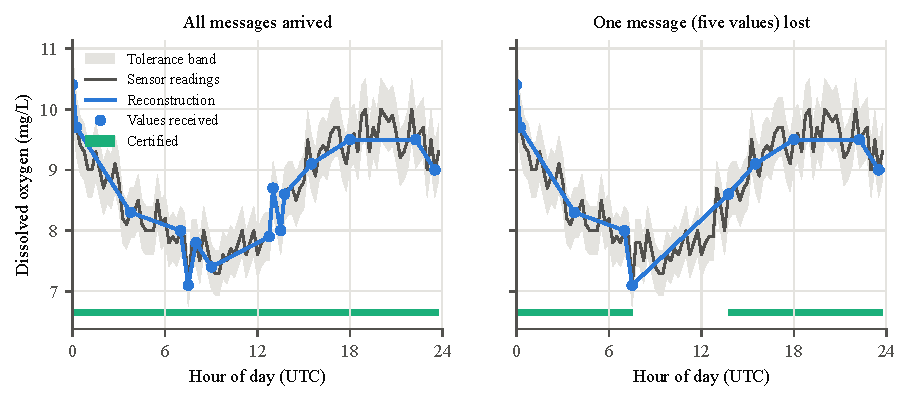
\includegraphics[width=\textwidth]{figs/example_day.pdf}
\caption{Dissolved oxygen on 1 July 2023 at a development site: the record (15 values in three messages) keeps every reading within tolerance; when the middle message is lost, the server certifies the readings outside the gap (bar) and leaves the gap uncertified.}
\label{fig:example}
\end{figure}

\begin{table}[t]
\centering
\caption{Environmental decisions at six messages per day (confirmation sites, four-parameter days). Decided: certainly exceeded or certainly not. Missed: exceedance days that the reconstruction, read naively, did not show.}
\label{tab:env}
\small
\begin{tabularx}{\textwidth}{@{}>{\raggedright\arraybackslash}X*{4}{>{\raggedright\arraybackslash}p{2.2cm}}@{}}
\toprule
Outcome & Record-first code & Record-first repetition & Every $k$-th reading & Tag practice \\
\midrule
\tableinput{tables/env.tex}
\bottomrule
\end{tabularx}
\end{table}

The record does not resolve features finer than its tolerance. pH exceedances in these data were mostly peaks one or two tenths above 9.0, against a tolerance of 0.2. A record within tolerance may flatten such a peak; therefore, read naively, it missed \missPHConf{} of \eventsPHConf{} pH exceedance days, against \missPHEveryConf{} for every $k$-th reading. The three-valued reading reports these days as undetermined rather than clear. For the same reason, periodic samples located the daily peak of dissolved oxygen and its diel range as well as the record did, or better (development data).

\subsection{Robustness}
\label{sec:robust}
Out-of-range readings were carried as censored flags: with one or three faulty readings injected per day, every day remained certifiable, at a cost of approximately \glitchCostDev{} values per faulty reading. Corruption of arriving messages acted as additional loss: at six messages per day the share of fully certified days fell from \corrNoneConf{} without corruption to \corrBerThreeConf{} at a bit-error rate of $10^{-3}$, with no reading certified outside its tolerance. At a bit-error rate of $10^{-2}$, where only 16\% of messages arrive intact, one corrupted parity message passed the CRC-16 by chance on one day and \falseCertConf{} readings were certified wrongly (Section~\ref{sec:confirm}). Removing record days did not change the bytes of any other day; therefore, outages do not propagate.

\subsection{Computational resources}
\label{sec:resources}
On the development data, the encoder needed a median of \opsFifteenDev{} window updates for a four-parameter day at 15-minute sampling and \opsFiveDev{} at 5 minutes, with memory proportional to the number of readings. Measured in Python on a desktop computer, it took a median of \hostFifteenS{}\,s and \hostFifteenKB{}\,kB of peak memory for a 15-minute day and \hostFiveS{}\,s and \hostFiveKB{}\,kB for a 5-minute day, against \hostTableFiveS{}\,s and \hostTableFiveMB{}\,MB for the reference implementation with a full error table; interpreter overhead dominates these times; therefore, the operation counts are the portable measure. At a conservative 200 processor cycles per update, a 48\,MHz microcontroller would encode a 5-minute day in approximately \mcuFiveDev{}\,s; the module's transmission energy, at most 2.5\,J per message \citep{kineis2023kim1}, exceeds the encoding energy by approximately three orders of magnitude. These figures are estimates; no microcontroller was used.

\subsection{Confirmation and temporal re-test}
\label{sec:confirm}
Six of the eight confirmatory hypotheses were supported (Table~\ref{tab:hyp}). C1 was not supported: the median record was \needMedConf{} bytes, within the predicted two messages, but the upper end of its interval (\needMedConfHi{} bytes) exceeded the 30-byte threshold, because the confirmation sites varied more than the development sites. C2 was not supported: on one of the \nDaysCorrConf{} days of the corruption experiment, at the highest bit-error rate tested, a corrupted parity message passed the CRC-16, an event expected approximately \collisionsExpConf{} times among the \crcChecksConf{} CRC checks of corrupted data at that error rate. The frozen receiver retried its erasure decoding over several parity combinations, and each retry is another chance for a corrupted message to pass a 16-bit check. After the confirmation, a corroboration rule was added: a decoding accepted only after an earlier attempt had failed must reproduce a received message that it did not use. A first attempt was left unchanged because it carries the same single-check risk as any received data unit. In an exploratory re-run of the corruption experiment on both cohorts, this rule removed every false certificate (\falseCertPostConf{} on the confirmation and \falseCertPostDev{} on the development sites) at a cost of \postCostThreeConf{} in the share of fully certified days at a bit-error rate of $10^{-3}$ and nothing without corruption. Under extreme corruption ($10^{-2}$), repetition then certified more days than the code (\postRepTwoConf{} against \postCodeTwoConf{}), because the code rejects decodings that it cannot corroborate.

Two low-cost deployments, opened in an earlier round of this study, were re-analysed after the confirmation as an exploratory check. On the InWaterSense node in Kosovo \citep{ahmedi2022} (\inwsDays{} four-parameter days), the record cost a median of \inwsMedBytes{} bytes, approximately 2.4 times the USGS median, and the code certified \inwsCodeSix{} of days at six messages per day (repetition \inwsRepSix{}) and \inwsCodeTwelve{} at twelve. On the Weija intake in Ghana \citep{adumanu2020} (temperature and conductance, \weijaDays{} days), the record cost \weijaMedBytes{} bytes and the code certified \weijaCodeSix{} of days at six messages per day (repetition \weijaRepSix{}). Noisy low-cost records therefore need larger plans; the small number of days makes these results indicative only.

On the 2024 data of the development sites (temporal re-test), the record-first code certified \gCodeIidRetest{} of days at six messages per day and $p = 0.3$, and the median record was \needMedRetest{} bytes; all eight criteria of Table~\ref{tab:hyp} were met, which is expected for sites whose 2023 data shaped the method and is therefore not counted as confirmation.
